% ===================== paper_main.tex (Article-style, concept-only) =====================
\documentclass[10pt]{article}

% --- Page setup ---
\usepackage[margin=1in]{geometry}
\usepackage{setspace} % optional
% \doublespacing % uncomment if needed

% --- Encoding & fonts ---
\usepackage[utf8]{inputenc}
\usepackage[T1]{fontenc}
\usepackage{lmodern}
\usepackage{microtype}

% --- Math / graphics / tikz / tables ---
\usepackage{amsmath, amssymb, amsthm, mathtools}
\usepackage{graphicx}
\usepackage{booktabs}
\usepackage{tikz}
\usetikzlibrary{shapes, arrows, positioning, calc}

% --- Hyperlinks ---
\usepackage{hyperref}
\hypersetup{colorlinks=true, linkcolor=blue, urlcolor=blue, citecolor=blue}

% --- Bibliography (choose one) ---
% Option A: natbib
\usepackage[numbers,sort&compress]{natbib}
% \bibliographystyle{unsrtnat}
% Option B: biblatex (comment natbib above and use backend=biber)
% \usepackage[backend=biber,style=numeric,sorting=none]{biblatex}
% \addbibresource{refs.bib}

% ===== Inline Icon Styles (match your figure styles exactly) =====
% 그림과 동일한 색/선/채움 사용
\tikzset{
  icon-mul/.style={draw, circle, fill=white, inner sep=0.8pt},
  icon-add-dashed/.style={draw, circle, dashed, fill=white, inner sep=0.6pt},
  icon-add-solid/.style={draw, circle, fill=white, inner sep=0.6pt},
  icon-aux/.style={draw, rectangle, fill=white, inner sep=1.2pt},
  icon-sum/.style={draw, circle, fill=white, inner sep=0.3pt}
}

% ===== Inline Icon Commands (use in text) =====
\newcommand{\iconMatMul}{%
  \tikz[baseline=-0.6ex]\node[icon-mul]{$\scriptsize\bullet$};%
}
\newcommand{\iconAddDashed}{%
  \tikz[baseline=-0.6ex]\node[icon-add-dashed]{\scriptsize$+$};%
}
\newcommand{\iconAddSolid}{%
  \tikz[baseline=-0.6ex]\node[icon-add-solid]{\scriptsize$+$};%
}
\newcommand{\iconAux}[1]{%
  \tikz[baseline=-0.6ex]\node[icon-aux]{\scriptsize #1};%
}
\newcommand{\iconSum}{%
  \tikz[baseline=-0.6ex]\node[icon-sum]{\tiny$\sum$};%
}


% --- Title & Authors ---
\title{Explainable Transformers via Graph-Based Operator Notation\\\large A Beginner-Oriented, Concept-Only Guide}
\author{Anonymous}
\date{} % add date if desired

% --- Theorem-like environments (optional) ---
\newtheorem{definition}{Definition}
\newtheorem{proposition}{Proposition}

% --- Unicode fallbacks for safety ---
\DeclareUnicodeCharacter{2295}{\ensuremath{\oplus}}      % ⊕
\DeclareUnicodeCharacter{2192}{\ensuremath{\rightarrow}} % →
\DeclareUnicodeCharacter{2219}{\ensuremath{\bullet}}     % •

\begin{document}
\maketitle

\begin{abstract}
We present a compact, pedagogy-first description of Transformers using a graph-based operator notation. Nodes denote operators, edges denote tensors, and double arrows mark the second operand of matrix multiplications. This article focuses on concepts (no code), pairing each formula with shape reasoning so a newcomer can translate diagrams into implementations after reading.\footnote{A practical, code-first companion is intentionally excluded in this version.}
This article is intentionally written for readers without prior neural-network background: it builds intuition first with operator–tensor diagrams, so that by the end one can follow the end-to-end Transformer flow, and later dive into the mathematical and implementation details with confidence.
\end{abstract}

\paragraph{Keywords} Transformer; attention; backpropagation; LayerNorm; softmax; diagram notation; pedagogy.

% ===================== 1. Introduction =====================
\section{Introduction}
Transformers have become the dominant sequence model in modern ML. However, many introductions assume prior exposure to neural networks and autodiff. We provide a beginner-friendly, concept-only path: (i) a concise section on graph notation and visual conventions, (ii) operator primitives with forward/backward summaries, (iii) multi-head attention (MHA) forward/backward, and (iv) assembly of a Transformer block (Input Embedding $\rightarrow$ MHA $\rightarrow$ MLP $\rightarrow$ Output Projection).
\paragraph{Learning Path and Promise}
We start from a visual, shape-first notation (Section~2), fix a small set of operator primitives with forward/backward summaries (Section~3), and then assemble the Transformer block from Input Encoding $\rightarrow$ MHA $\rightarrow$ MLP $\rightarrow$ Output Projection (Sections~4–5).
By design, a reader who “doesn’t yet know where to start” can still finish with a working mental model of the full Transformer flow, and later return to fill in mathematics, cost models, and implementation details without losing the big picture.

\subsection{Contributions}
(1) A consistent diagrammatic convention that separates operators from data. (2) Shape-first backprop summaries, including broadcasting and reduce axes. (3) A compact Transformer walkthrough suitable for first-time readers.

\section{Graph Notation and Visual Conventions}
\paragraph{How to Read This Section}
If you feel lost about where to begin, read this section as a map: each icon in the figures has a one-to-one meaning here (node type, edge role, and shape tags).
Once you can read a single forward figure and a single backward figure fluently, the entire Transformer flow becomes a sequence of these same primitives reused in different places.

We use operator–tensor graphs where nodes are operators and edges carry tensors. The notation is identical in text and figures to avoid ambiguity and testing mismatches.

\subsection{Node Types (exactly as in figures)}
\begin{itemize}
  \item \textbf{MatMul} \iconMatMul\ : green circular node with a centered $\bullet$ (matrix multiplication).
  \item \textbf{Elementwise Add / Bias Add} \iconAddDashed\ : red dashed circle with a centered $+$ (broadcasting allowed).
  % If you chose solid style instead, swap to \iconAddSolid
  \item \textbf{Nonlinear / Normalization / Utility} \iconAux{LN}, \iconAux{GL}, \iconAux{DO}, \iconAux{T}, \iconAux{S}, \iconAux{SM}, \iconAux{CE}:
        yellow rectangle with the operator label (LayerNorm, GELU, Dropout, Transpose, Softmax, Score+Mask, Cross-Entropy).
  \item \textbf{Reduction} \iconSum\ : small red circle with $\sum$ (axis reductions such as $\sum_{B,S}$ for bias gradients).
\end{itemize}

\subsection{Edges and the Double-Arrow Convention}
We draw one diagram per direction. In a forward diagram, all arrows carry forward values; in a backward diagram, all arrows carry gradients. We therefore use one unified arrow style:
\begin{itemize}
  \item \textbf{Value flow:} single solid arrow $\to$ for all tensors in the current diagram.
  \item \textbf{Second MatMul operand:} double arrow $\Rightarrow$ into the MatMul node to mark the right-hand matrix (e.g., weights, possibly transposed).
  \item \textbf{Reductions:} a \iconSum\ node denotes axis reductions (e.g., $\sum_{B,S}$).
\end{itemize}
The double arrow removes ambiguity about which factor is on the right in $Z=XW$, and clarifies where transposes appear in backprop.

\subsection{Tensor Names, Shapes, and Broadcasting}
Edges are labeled with names and shapes, e.g., $[B,S,D]$, $[B,S,D_{\mathrm{ff}}]$.
Broadcast notation $\mathrm{BC}_{B,S}(\cdot)$ indicates expansion (e.g., $\mathrm{BC}_{B,S}(\tilde{\mathbf{b}}_{\text{up}}):[D_{\mathrm{ff}}]\to[B,S,D_{\mathrm{ff}}]$).

\subsection{MatMul Orientation and Backprop}
For $Z=XW$ we mark $W$ with the double arrow. Backprop uses
\[
\frac{\partial L}{\partial X}=G\,W^{\top},\qquad
\frac{\partial L}{\partial W}=X^{\top}G,
\]
with $G=\partial L/\partial Z$. In diagrams, needed transposes are shown with \iconAux{T} before the gradient-accumulation MatMul.

\subsection{Bias Add and Reductions}
For $Y=A+B$ with broadcasting, the gradient w.r.t.\ $B$ reduces across broadcast axes:
\[
\frac{\partial L}{\partial B}=\sum_{\text{broadcast axes}} \frac{\partial L}{\partial Y}.
\]
We render this with a \iconSum\ node labeled $\sum_{B,S}$ at bias-add sites.

\subsection{(Optional) Cost Badges}
You may attach small badges: \texttt{FLOPs=} inside MatMul nodes (e.g., $2mkn$) and \texttt{[shape $|$ bytes]} on wide edges, to immediately surface compute/memory hot spots.


% ===================== 3. Operator Primitives =====================
\section{Operator Primitives}
\subsection{General Backprop Rule for $z=f(x,y)$}
Let $g = \partial L/\partial z$. Then
\begin{equation}
\frac{\partial L}{\partial x} = \texttt{reduce\_like}\big(g\odot \tfrac{\partial f}{\partial x},\; x\big),\quad
\frac{\partial L}{\partial y} = \texttt{reduce\_like}\big(g\odot \tfrac{\partial f}{\partial y},\; y\big),
\end{equation}
where \texttt{reduce\_like} sums over broadcast axes to match the input shape. For MatMul $Z=AB$ with upstream $G$, $\partial L/\partial A=GB^{\top}$ and $\partial L/\partial B=A^{\top}G$.

\subsection{Elementwise Add / Bias Add}
$Y=A+B$. Gradients reduce along broadcast axes.

\subsection{Linear / Projection}
$Y= XW + b$. $\partial L/\partial X=(\partial L/\partial Y)W^{\top}$, $\partial L/\partial W=X^{\top}(\partial L/\partial Y)$, $\partial L/\partial b=\sum\limits_{B,S}(\partial L/\partial Y)$.

\subsection{Softmax (Stable)}
With $Y=\text{softmax}(Z)$ along the last axis, $\partial L/\partial Z=(G-\langle G,Y\rangle)\odot Y$, where $G=\partial L/\partial Y$ and the inner product is along the softmax axis.

\subsection{LayerNorm (LN)}
Summarize forward $(\mu,\sigma,\hat X)$ and use the standard derivative form with cached statistics.

% ===================== 4. Multi-Head Attention =====================
\section{Multi-Head Attention (MHA)}
\subsection{Forward}
Given $Q,K,V\in\mathbb{R}^{[B,H,S,D_h]}$, scores $A=QK^{\top}/\sqrt{D_h}$, probabilities $P=\text{softmax}(A)$ (with masking), outputs $O=PV$. Heads are merged (concat) and projected. Shapes: $A,P\in\mathbb{R}^{[B,H,S,S]}$, $O\in\mathbb{R}^{[B,S,D]}$.

\subsection{Backward (Summary)}
$dO\rightarrow dV=P^{\top}dO$, $dO\rightarrow dP=dO\,V^{\top}$, $dP\rightarrow dA=(dP-\text{sum}(dP\odot P))\odot P$, masking zeros gradients on masked entries, and $dA\rightarrow dQ=dA\,K/\sqrt{D_h}$, $dA\rightarrow dK=dA^{\top}Q/\sqrt{D_h}$.

% ===================== 5. Transformer Block =====================
\section{Transformer Block (Concept-Only)}
\textbf{Pipeline}: Input Embedding $\rightarrow$ MHA $\rightarrow$ MLP (FFN) $\rightarrow$ Output Projection, with residual connections and LayerNorm.\\
\textbf{Input Embedding}: token table $E\in\mathbb{R}^{V\times D}$ mapping $[B,S]$ to $[B,S,D]$; positional signal (absolute/learned or RoPE).\\
\textbf{MLP}: Linear--GELU--Linear (or SwiGLU), expansion factor $\alpha$.\\
\textbf{Output Projection}: logits via $W_{lm}\in\mathbb{R}^{D\times V}$; optionally tie with $E$.

% ===================== 6. Figures (placeholders) =====================
\section{Figures}
% Example figure environment (replace with your TikZ)
\begin{figure}[h]
  \centering
  % \resizebox{\linewidth}{!}{%
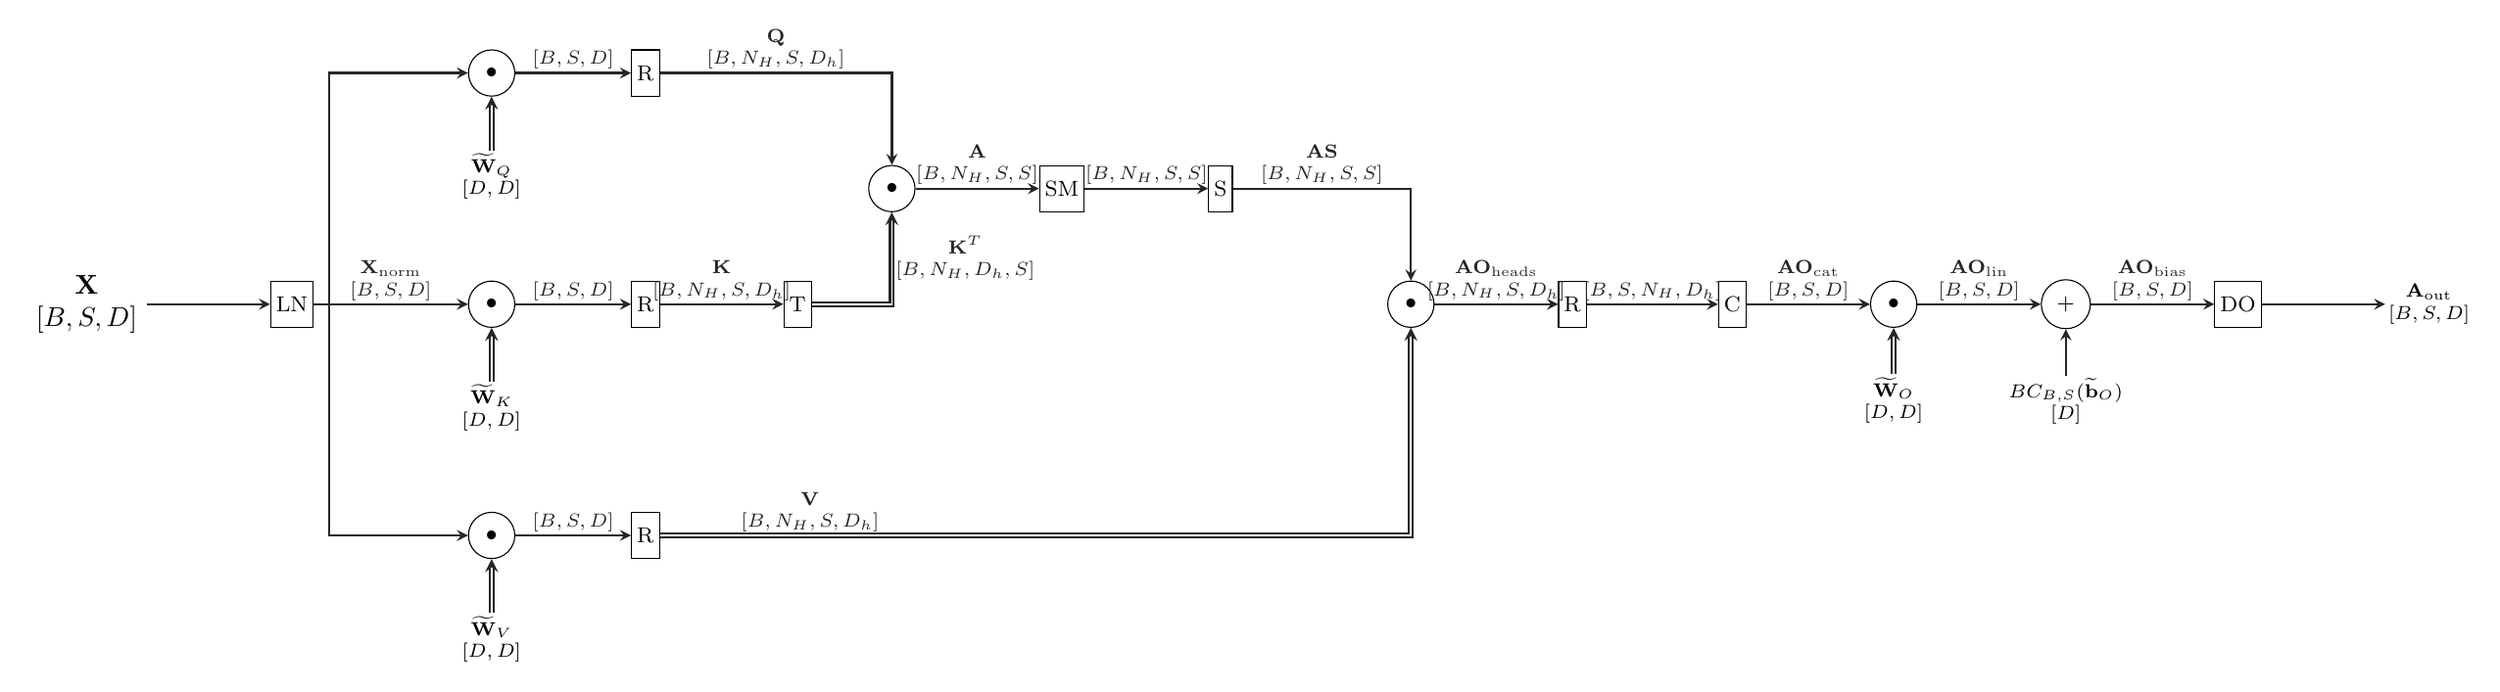
\begin{tikzpicture}[
  every node/.style={transform shape},
  >=stealth,
  auxnode/.style={draw, rectangle, fill=white, minimum height=6mm, inner sep=2pt, font=\footnotesize, align=center},
  mulnode/.style={draw, circle, fill=white, minimum size=6mm, font=\footnotesize, align=center},
  addnode/.style={draw, circle, fill=white, minimum size=6mm, font=\footnotesize, align=center},
  flow/.style={->, thick, black!85},
  flow2/.style={->, double, thick, black!85},
  dimlabel/.style={font=\scriptsize, inner sep=1pt, align=center}
]
% \node[font=\Large\bfseries] at (8, 4.5) {Multi-Head Attention Forward Pass};

\node (Input) at (0.5, 0) [align=center] {$\mathbf{X}$\\$[B,S,D]$};
\node[auxnode] (LN) [right=1.6cm of Input] {LN};

\node[mulnode] (Proj_Q) [right=2.0cm of LN, yshift=3.0cm] {$\bullet$};
\node[auxnode] (R_Q) [right=1.5cm of Proj_Q] {R};

\node[mulnode] (Proj_K) [right=2.0cm of LN, yshift=0cm] {$\bullet$};
\node[auxnode] (R_K) [right=1.5cm of Proj_K] {R};

\node[mulnode] (Proj_V) [right=2.0cm of LN, yshift=-3.0cm] {$\bullet$};
\node[auxnode] (R_V) [right=1.5cm of Proj_V] {R};

\node[dimlabel] (WQ) [align=center, below=0.7cm of Proj_Q] {$\widetilde{\mathbf{W}}_{Q}$\\$[D,D]$};
\node[dimlabel] (WK) [align=center, below=0.7cm of Proj_K] {$\widetilde{\mathbf{W}}_{K}$\\$[D,D]$};
\node[dimlabel] (WV) [align=center, below=0.7cm of Proj_V] {$\widetilde{\mathbf{W}}_{V}$\\$[D,D]$};

\node[auxnode] (T_K) [right=1.6cm of R_K] {T};
\node[mulnode] (QK) [right=2.7cm of R_Q, yshift=-1.5cm] {$\bullet$};
\node[auxnode] (SM) [right=1.6cm of QK] {SM};
\node[auxnode] (Soft) [right=1.6cm of SM] {S};
\node[mulnode] (PV) [right=2.0cm of Soft, yshift=-1.5cm] {$\bullet$};

\node[auxnode] (R_Merge) [right=1.6cm of PV] {R};
\node[auxnode] (Cat) [right=1.7cm of R_Merge] {C};

\node[mulnode] (OProj) [right=1.6cm of Cat] {$\bullet$};
\node[dimlabel] (WO_FWD) [align=center, below=0.6cm of OProj] {$\widetilde{\mathbf{W}}_{O}$\\$[D,D]$};
\node[addnode] (AddB) [right=1.6cm of OProj] {+};
\node[dimlabel] (BO) [align=center, below=0.6cm of AddB] {$BC_{B,S}(\widetilde{\mathbf{b}}_{O})$\\$[D]$};
\node[auxnode] (Drop) [right=1.6cm of AddB] {DO};
\node[dimlabel] (Aout) [align=center, right=1.6cm of Drop] {$\mathbf{A}_{\text{out}}$\\$[B,S,D]$};

\draw[flow] (Input) -- (LN);

\draw[flow] (LN.east) -- ++(0.2,0) |- (Proj_Q.west);
\draw[flow] (LN) -- (Proj_K.west) node[dimlabel, midway, above]{$\mathbf{X}_{\text{norm}}$\\$[B,S,D]$};
\draw[flow] (LN.east) -- ++(0.2,0) |- (Proj_V.west);

\draw[flow2] (WQ) -- (Proj_Q);
\draw[flow2] (WK) -- (Proj_K);
\draw[flow2] (WV) -- (Proj_V);

\draw[flow] (Proj_Q) -- (R_Q) node[dimlabel, midway, above]{$[B,S,D]$};
\draw[flow] (Proj_K) -- (R_K) node[dimlabel, midway, above]{$[B,S,D]$};
\draw[flow] (Proj_V) -- (R_V) node[dimlabel, midway, above]{$[B,S,D]$};

\draw[flow] (R_Q) -| (QK) node[dimlabel, near start, above]{$\mathbf{Q}$\\$[B,N_H,S,D_h]$};
\draw[flow] (R_K) -- (T_K) node[dimlabel, midway, above]{$\mathbf{K}$\\$[B,N_H,S,D_h]$};
\draw[flow2] (T_K) -| (QK) node[dimlabel, near end, right]{$\mathbf{K}^{T}$\\$[B,N_H,D_h,S]$};

\draw[flow] (QK) -- (SM) node[dimlabel, midway, above]{$\mathbf{A}$\\$[B,N_H,S,S]$};
\draw[flow] (SM) -- (Soft) node[dimlabel, midway, above]{$[B,N_H,S,S]$};
\draw[flow] (Soft) -| (PV) node[dimlabel, near start, above]{$\mathbf{AS}$\\$[B,N_H,S,S]$};
\draw[flow2] (R_V) -| (PV) node[dimlabel, pos=0.1, above]{$\mathbf{V}$\\$[B,N_H,S,D_h]$};

\draw[flow] (PV) -- (R_Merge) node[dimlabel, midway, above]{$\mathbf{AO}_{\text{heads}}$\\$[B,N_H,S,D_h]$};
\draw[flow] (R_Merge) -- (Cat) node[dimlabel, midway, above]{$[B,S,N_H,D_h]$};
\draw[flow] (Cat) -- (OProj) node[dimlabel, midway, above]{$\mathbf{AO}_{\text{cat}}$\\$[B,S,D]$};
\draw[flow2] (WO_FWD) -- (OProj);
\draw[flow] (OProj) -- (AddB) node[dimlabel, midway, above]{$\mathbf{AO}_{\text{lin}}$\\$[B,S,D]$};
\draw[flow] (BO) -- (AddB);
\draw[flow] (AddB) -- (Drop) node[dimlabel, midway, above]{$\mathbf{AO}_{\text{bias}}$\\$[B,S,D]$};
\draw[flow] (Drop) -- (Aout);
\end{tikzpicture}%
}
 % if externalized
  \caption{Forward pass of multi-head attention using the proposed legend.}
  \label{fig:mha-forward}
\end{figure}

% ===================== 7. Discussion & Limitations =====================
\section{Discussion and Limitations}
Scope is conceptual; we omit code, datasets, and training details. Numerical stability notes (softmax, LN) are summarized rather than proven.

% ===================== 8. Conclusion =====================
\section{Conclusion}
We deliberately prioritized a diagram-first, beginner-friendly path so that readers without a neural-network background can still form a correct end-to-end mental model of Transformers.
From here, the same operator–tensor vocabulary extends naturally to stability tricks (e.g., log-sum-exp, pre-LN), cost models (FLOPs/bytes per edge), training regimes, and implementation details (fused kernels, KV caching), without losing the overall flow.

% ===================== References =====================
% natbib example:
% \bibliography{refs}

% biblatex example:
% \printbibliography

\end{document}
